\chapter{CellTAN Application}

\section{MPPT Curve}

\begin{figure}[h]
    \centering
    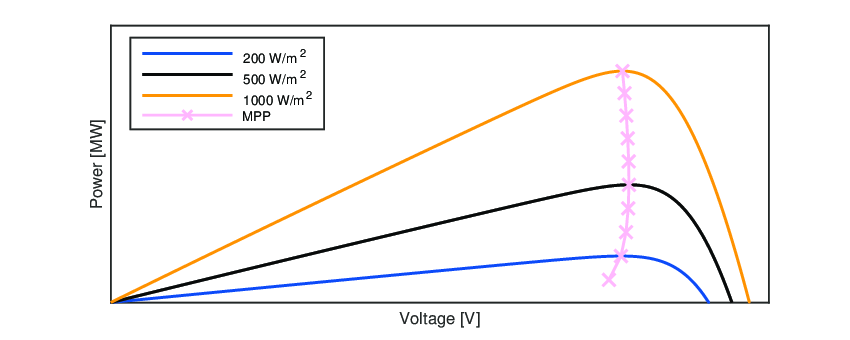
\includegraphics[width=14cm]{figures/appendix/b_analysis/mpptcurve.png} \caption{"PV panel power characteristics as a function of the DC voltage and solar irradiance."} Image source and copyright: \cite{lunardi}.
    \label{fig:mpptcurve}
\end{figure}

\FloatBarrier
\section{Data Analysis} \label{ap2:eda}

\begin{figure}[h]
    \centering
    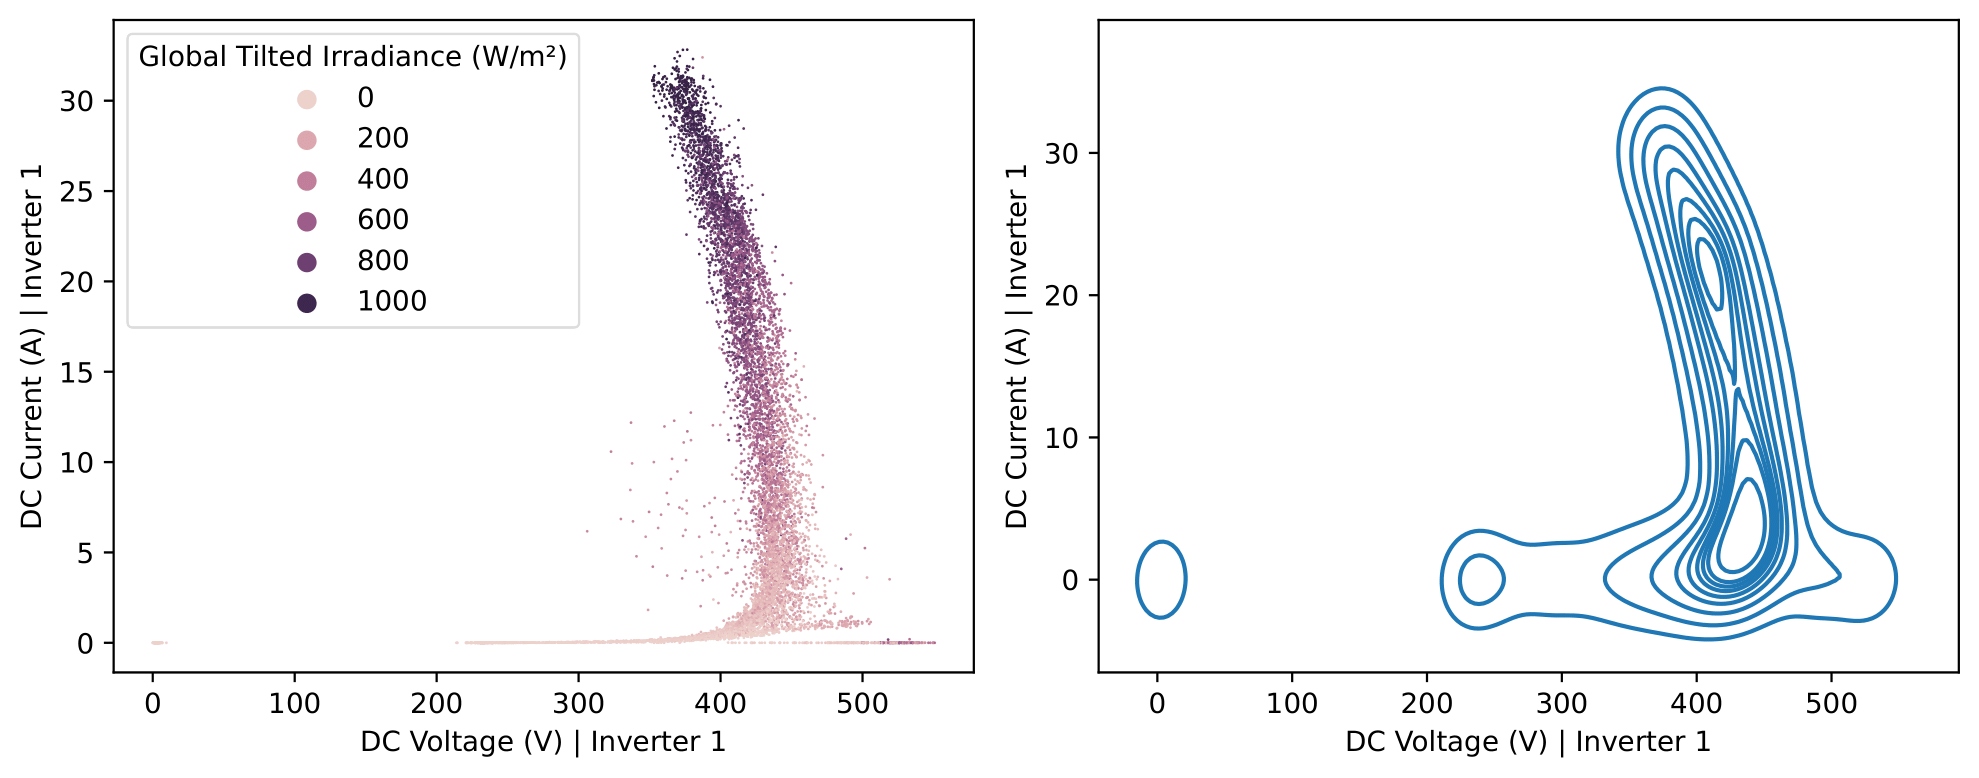
\includegraphics[width=\textwidth]{figures/appendix/b_analysis/05_voltage_current_pairplot_test_1-1.png}
    \caption{Pair plot of DC side voltage and current from inverter one (2023), using scatter (left) and KDE (Kernel Density Estimation) (right).}
    \label{fig:eda_voltage_current_test_1}
\end{figure}

\begin{figure}[h]
    \centering
    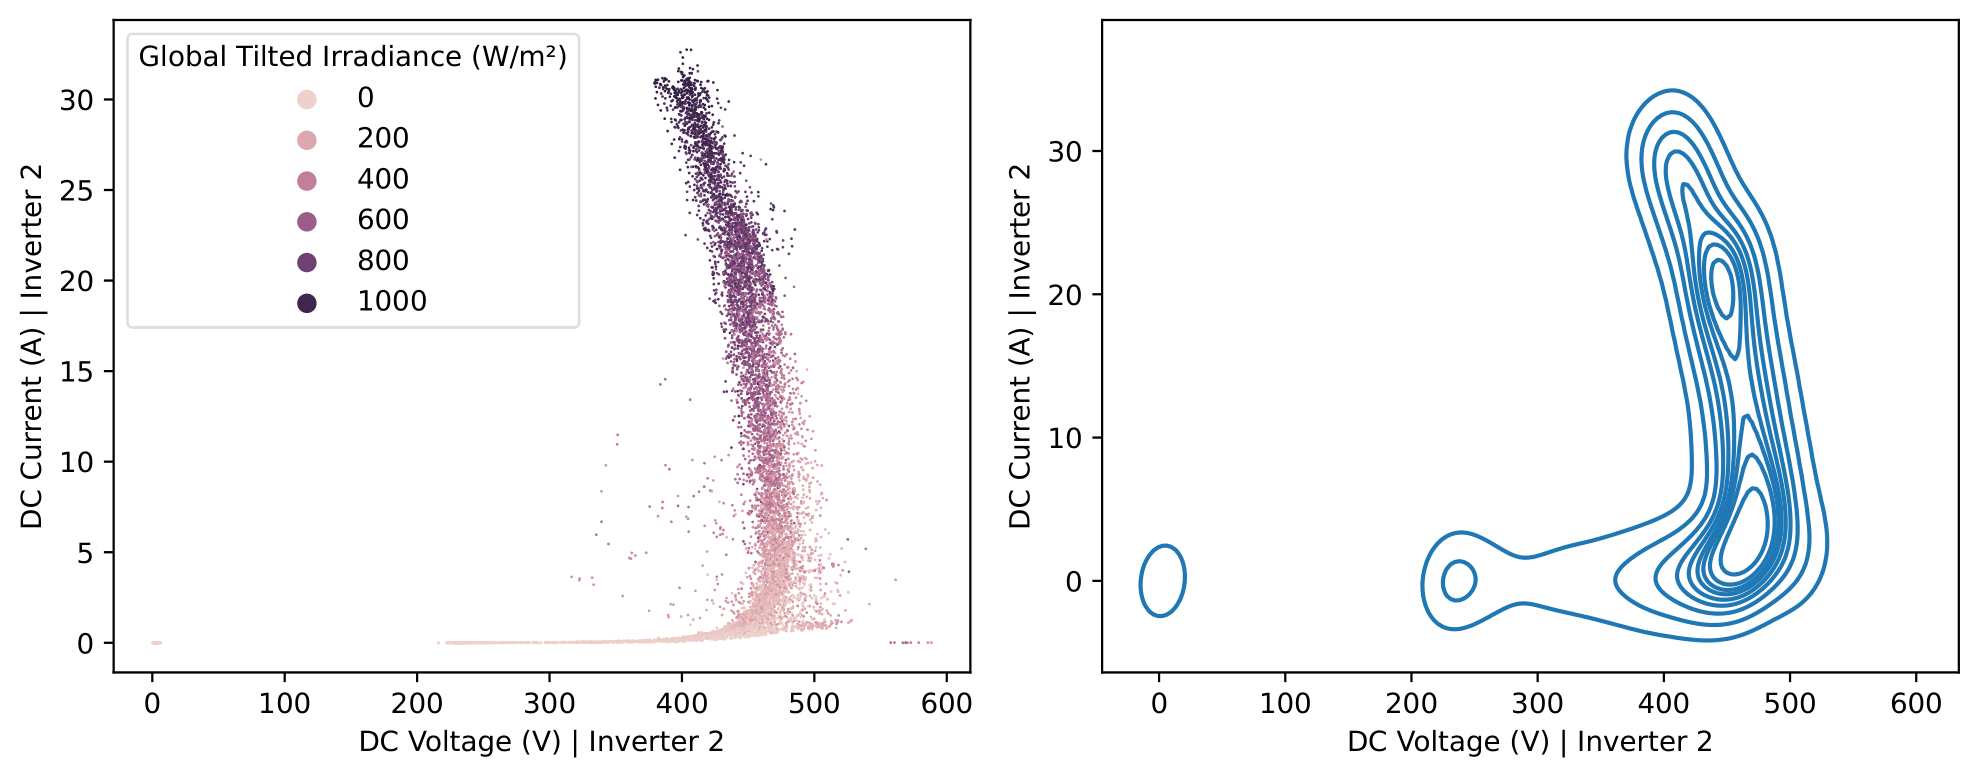
\includegraphics[width=\textwidth]{figures/appendix/b_analysis/07_voltage_current_pairplot_test_2-1.png}
    \caption{Pair plot of DC side voltage and current from inverter two (2023), using scatter (left) and KDE (Kernel Density Estimation) (right).}
    \label{fig:eda_voltage_current_test_2}
\end{figure}

\begin{figure}[h]
    \centering
    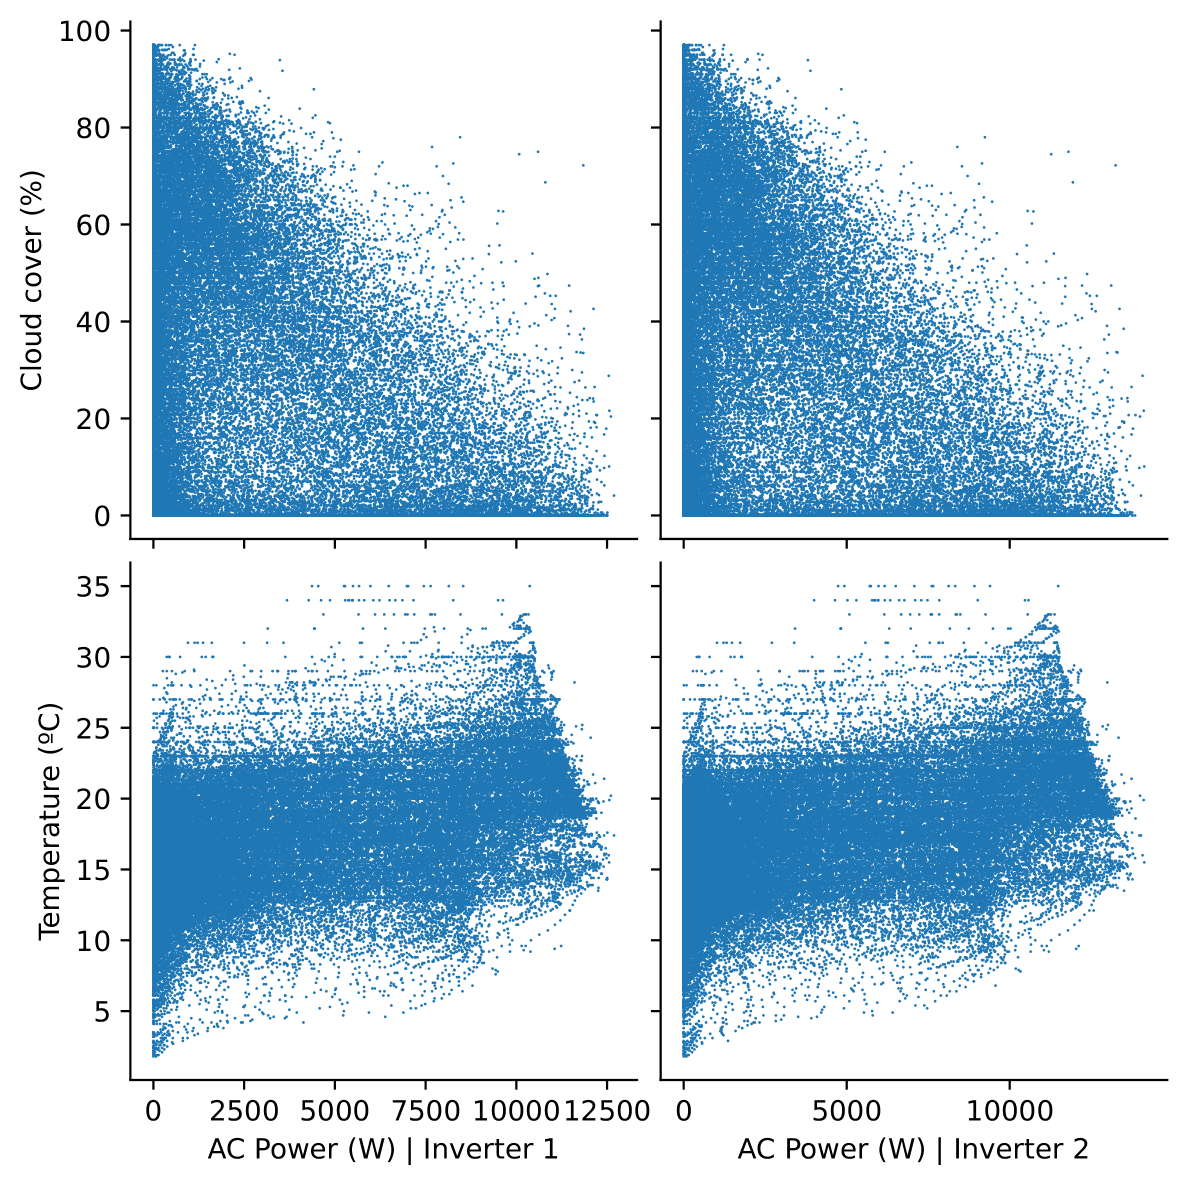
\includegraphics[width=0.6\textwidth]{figures/appendix/b_analysis/12_power_meteo_pairplot_kb-1.png}
    \caption{Scatter pair-plot of AC power from the two inverters with cloud coverage and temperature (from satellite).}
    \label{fig:eda_irrelevant_meteo}
\end{figure}

\FloatBarrier

\section{Data Cleaning}

\subsection{Satellite}

\begin{figure}[h!]
    \centering
    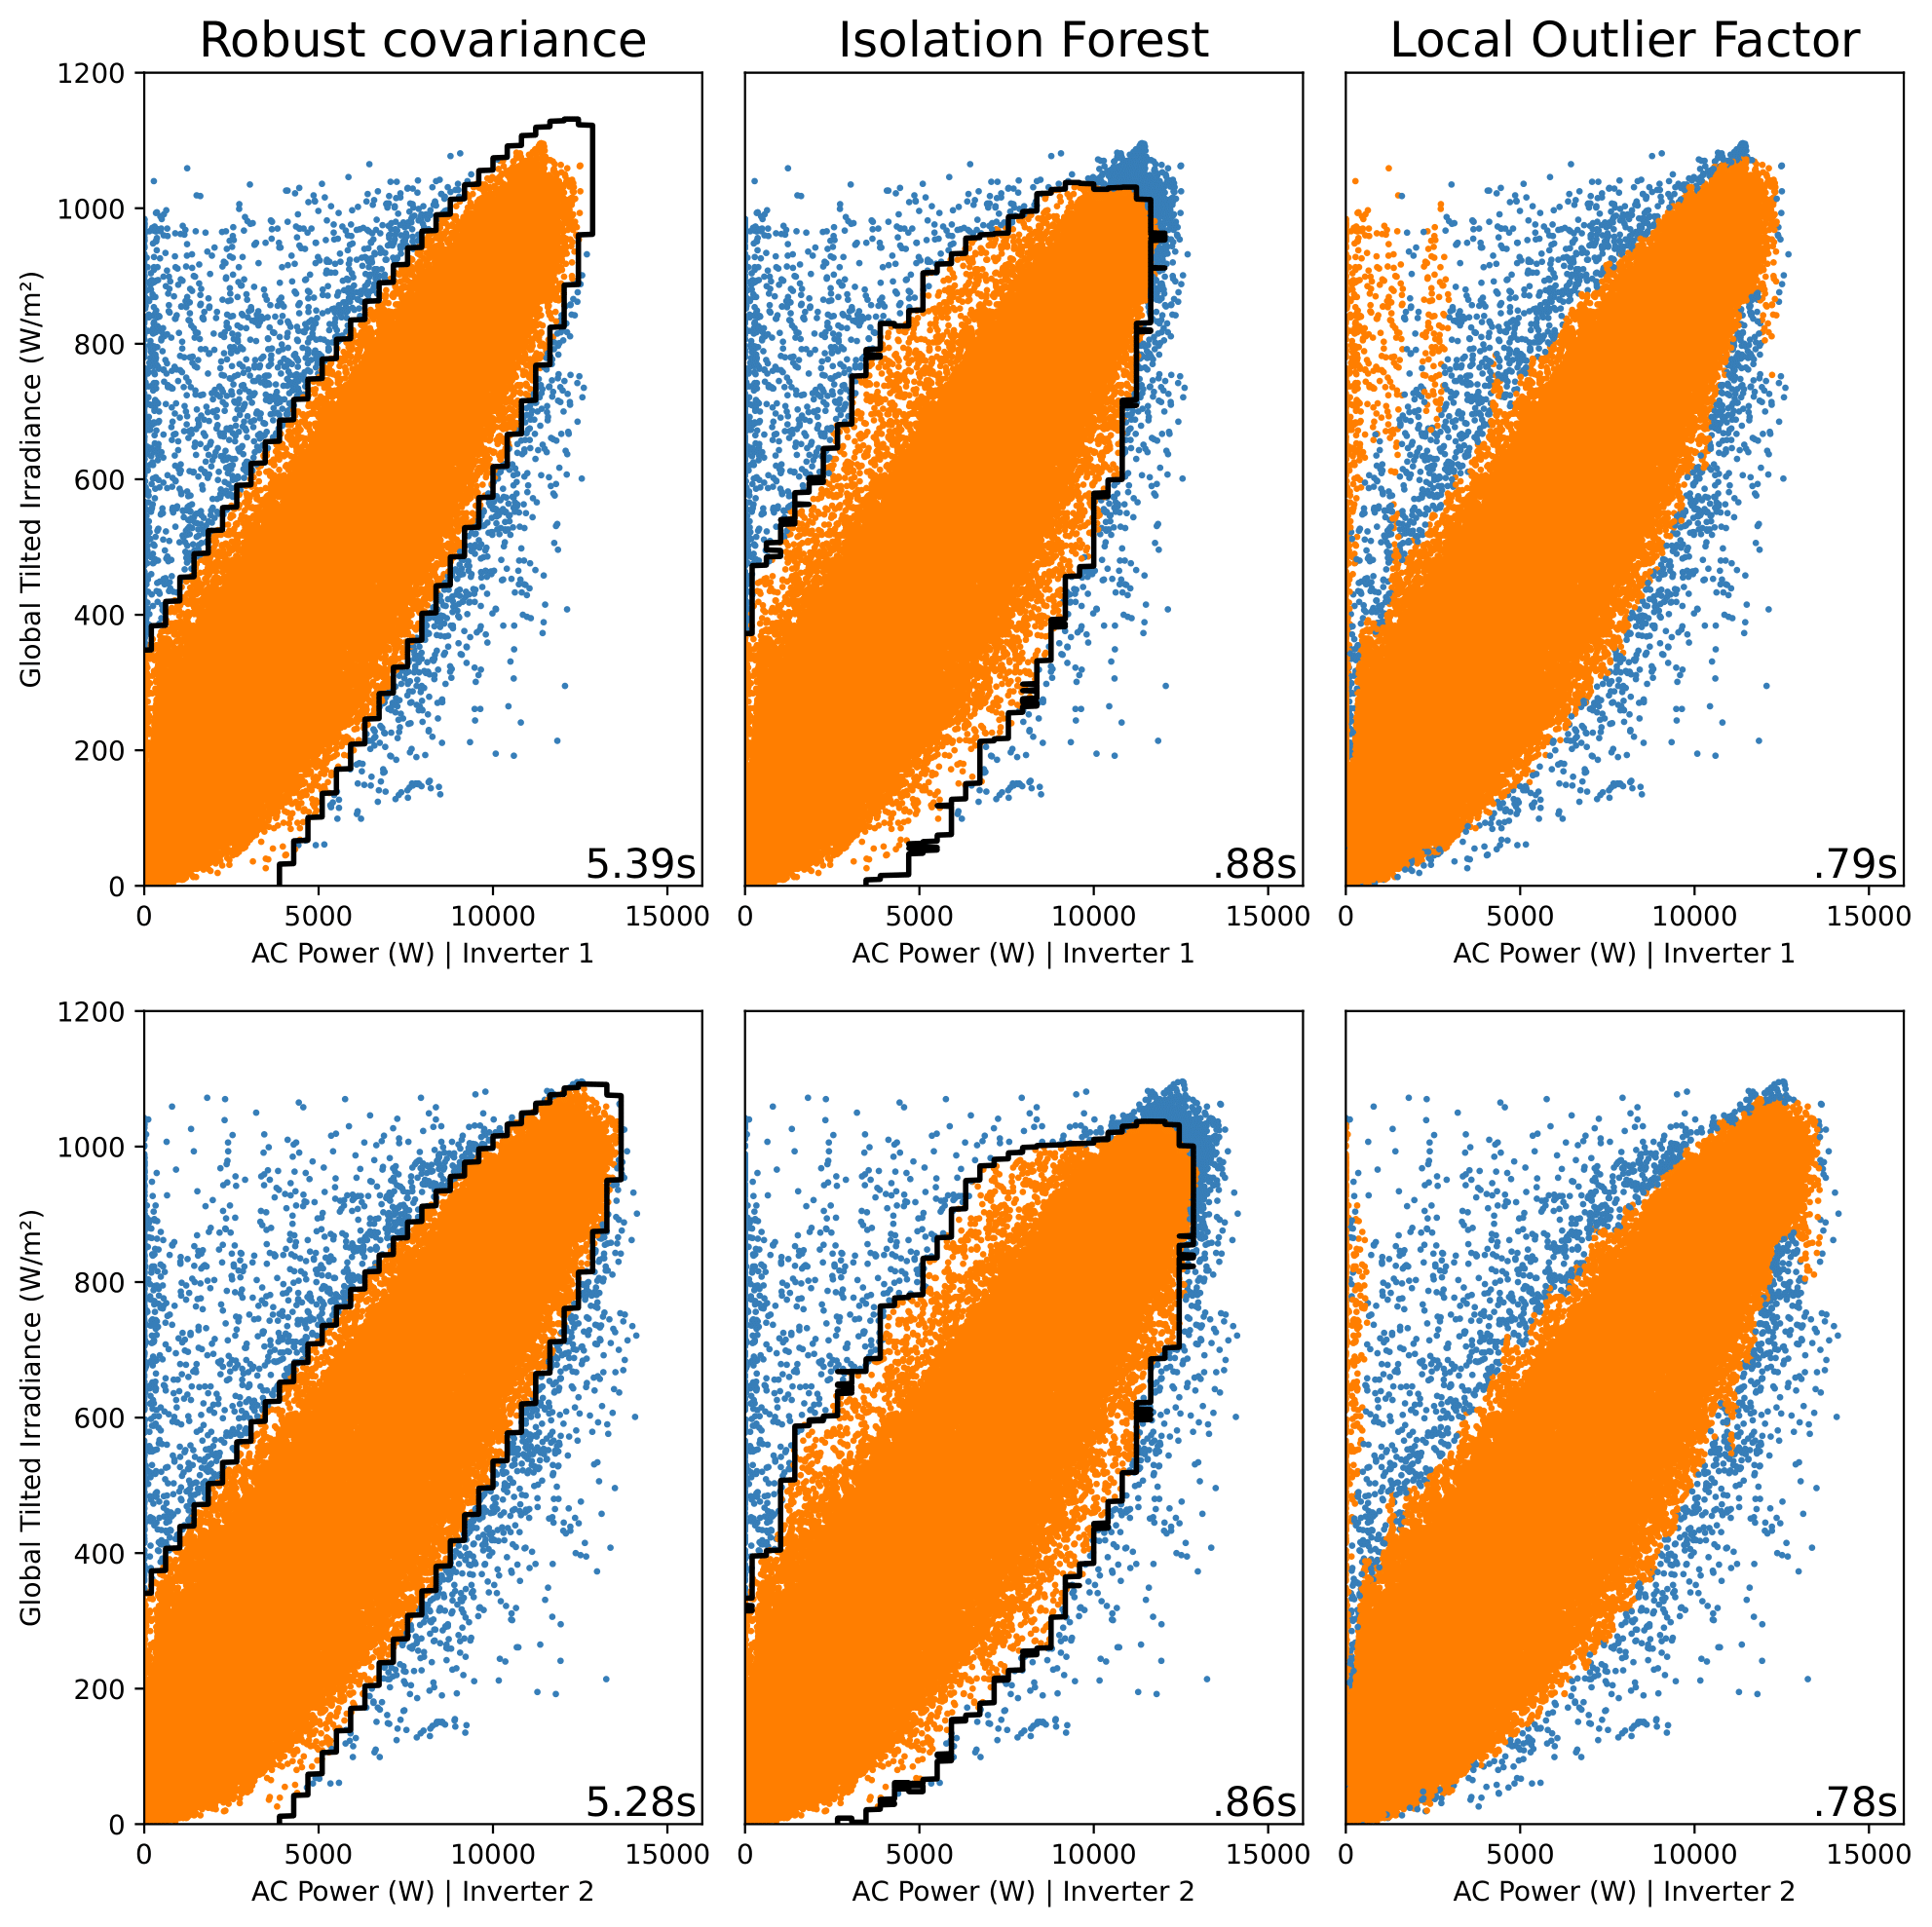
\includegraphics[width=\textwidth]{figures/appendix/b_analysis/21_cleaning_tilted_irrad-1.png}
    \caption{Inliers (orange), outliers (blue), and decision boundaries (black) using three different anomaly detection algorithms on the tilted irradiance and AC Power from both inverters.}
    \label{fig:clean_tilted_irrad}
\end{figure}

\begin{figure}[h!]
    \centering
    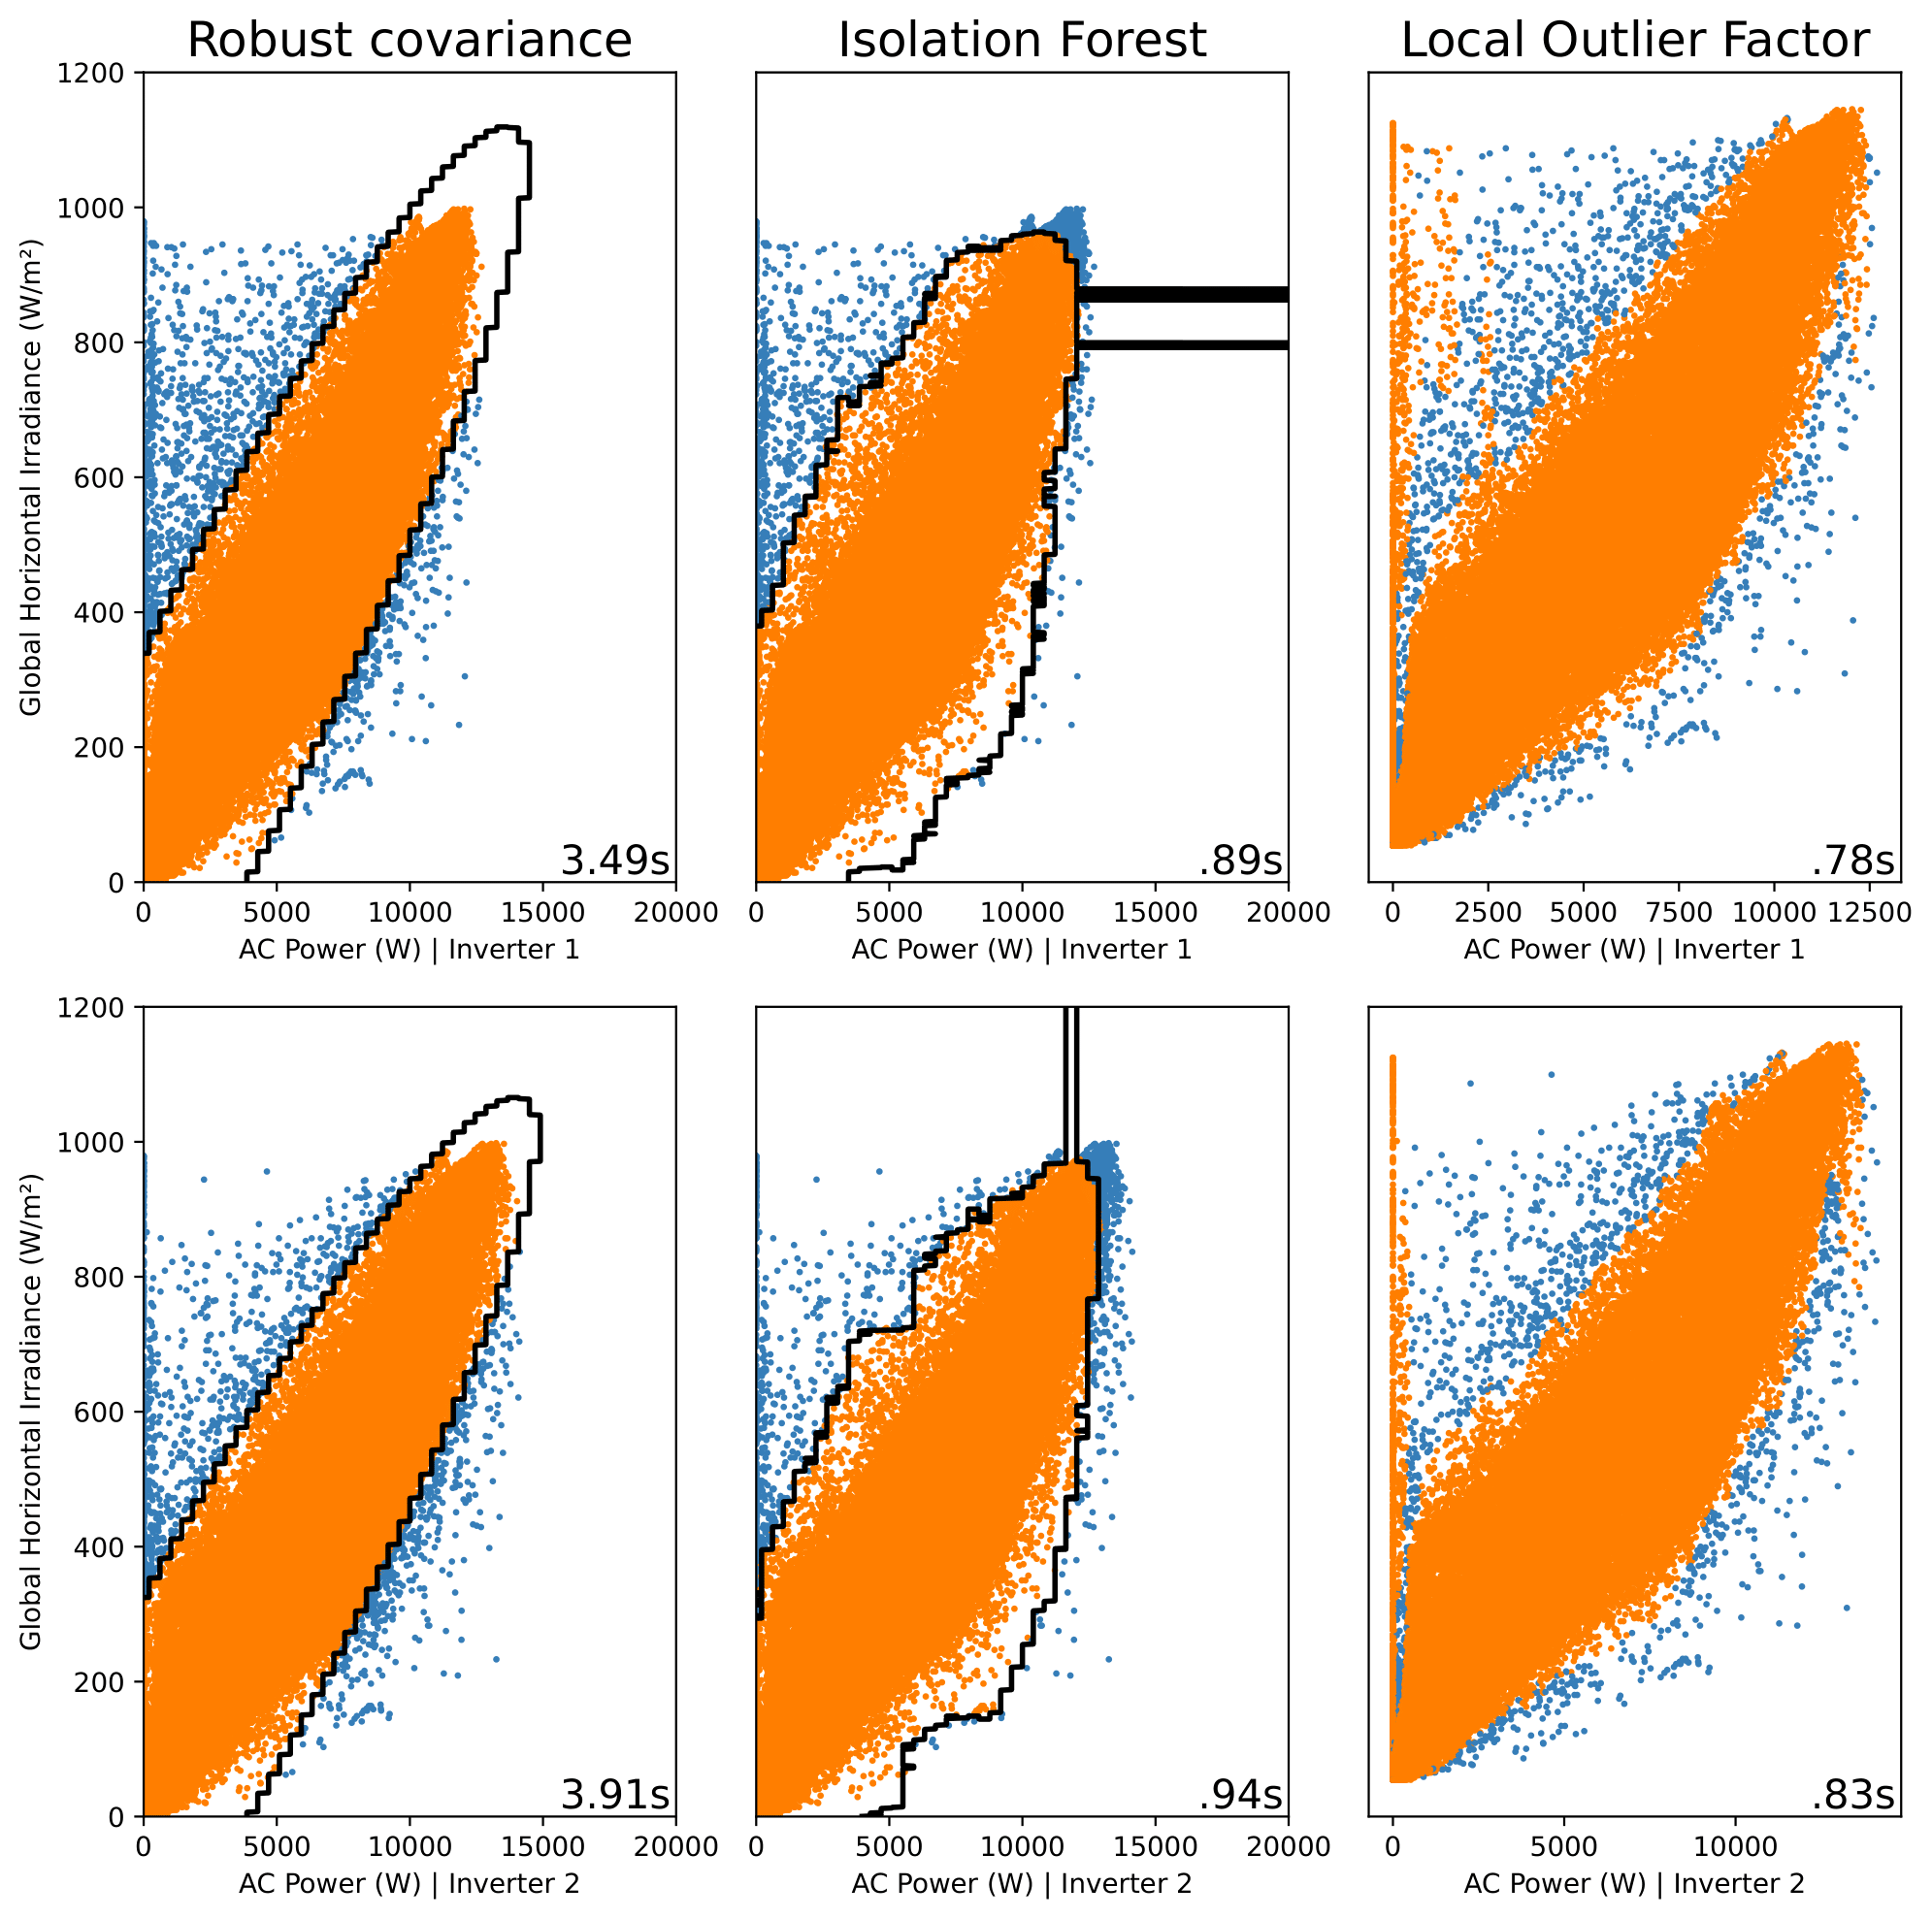
\includegraphics[width=\textwidth]{figures/appendix/b_analysis/22_cleaning_horizontal_irrad-1.png}
    \caption{Inliers (orange), outliers (blue), and decision boundaries (black) using three different anomaly detection algorithms on the horizontal irradiance and AC Power from both inverters.}
    \label{fig:clean_horizontal_irrad}
\end{figure}

\subsection{Voltage and Current}

\begin{figure}[h!]
    \centering
    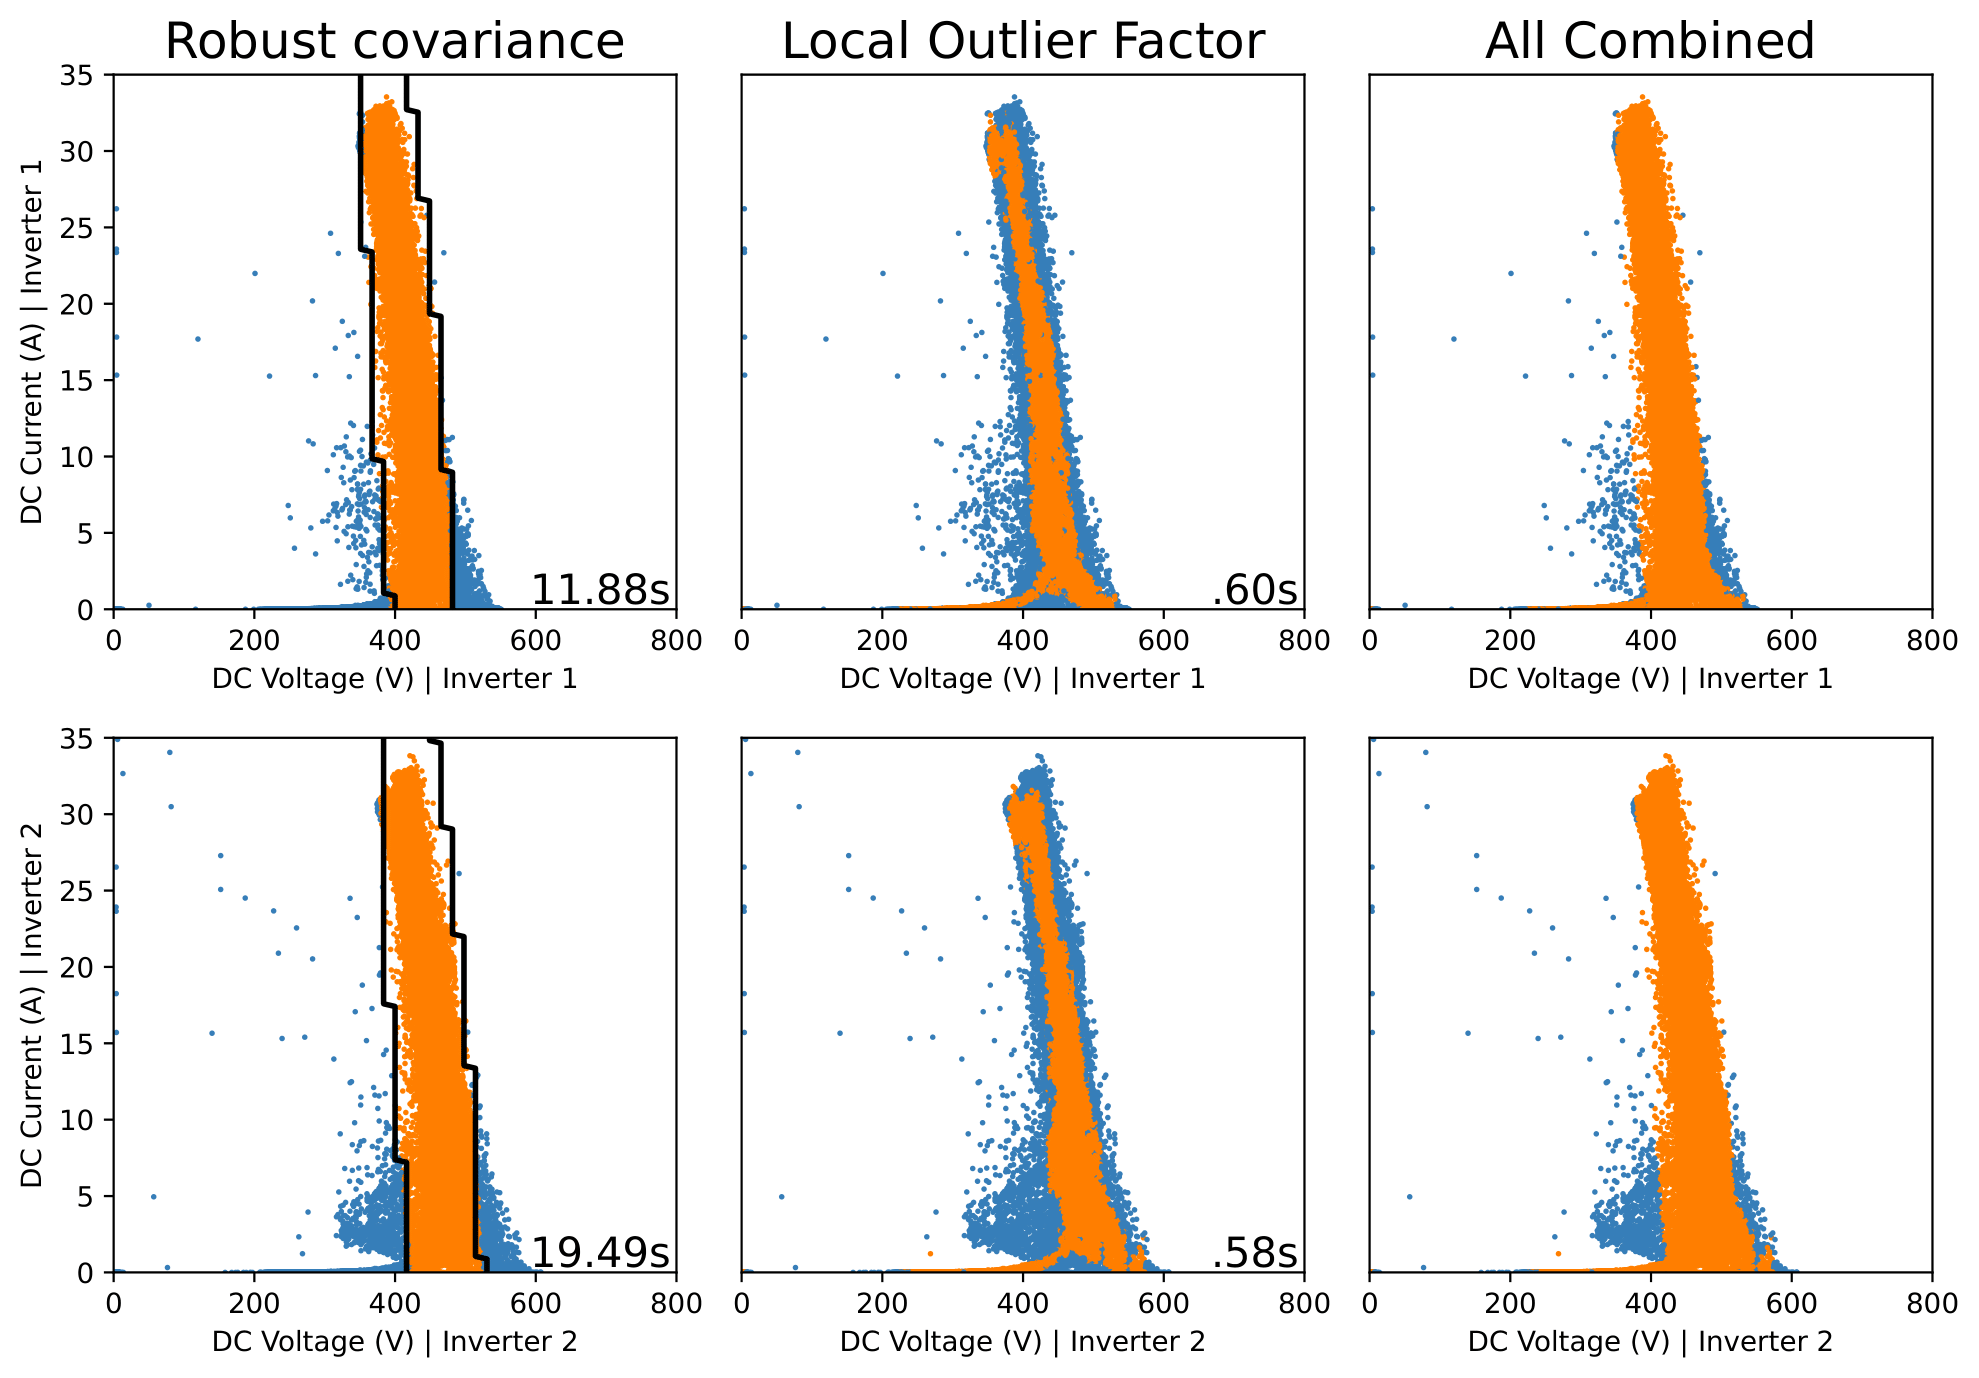
\includegraphics[width=\textwidth]{figures/appendix/b_analysis/23_cleaning_volt_curr-1.png}
    \caption{Inliers (orange), outliers (blue), and decision boundaries (black) using two different anomaly detection algorithms and their combination on the DC side voltage and current from both inverters.}
    \label{fig:clean_volt_curr}
\end{figure}

\FloatBarrier

\section{Photovoltaic Plugin}

\begin{figure}[h!]
    \centering
    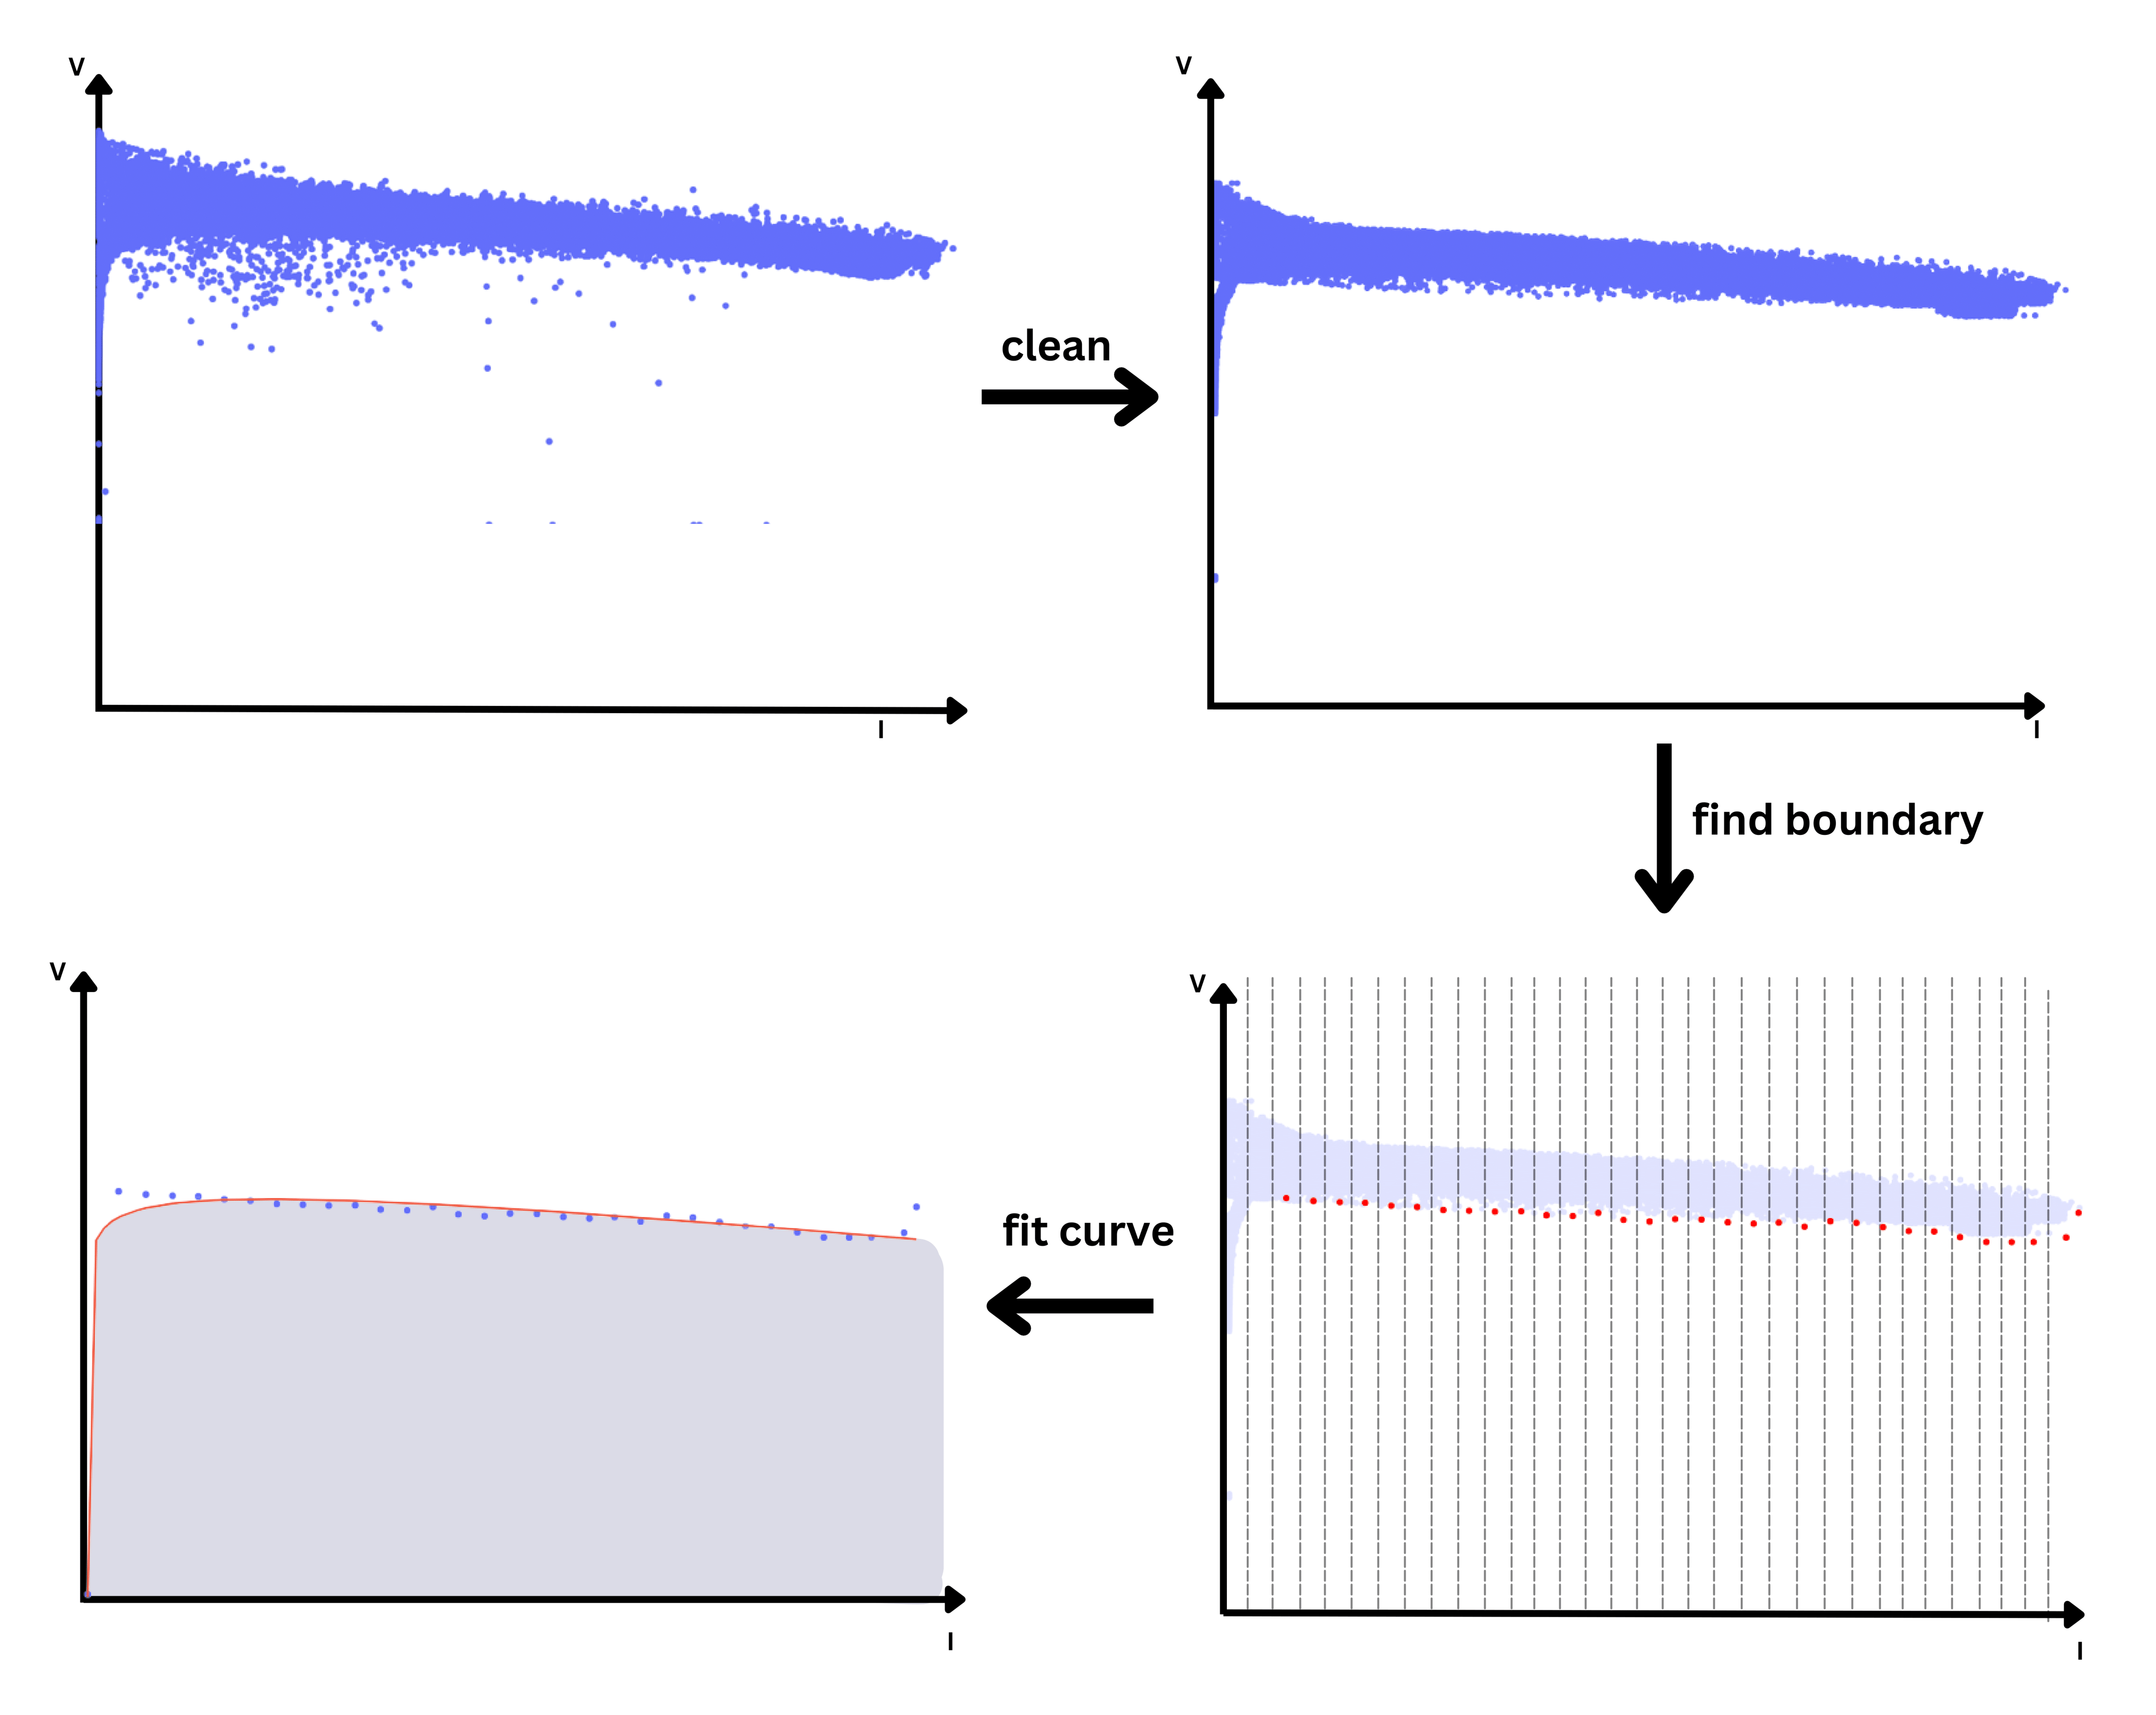
\includegraphics[width=0.8\textwidth]{figures/appendix/b_analysis/plugin_steps-1.png}
    \caption{Proposed steps for obtaining inverter underperformance region.}
    \label{fig:pluginsteps}
\end{figure}

\FloatBarrier

\section{Cell Configuration}  \label{ap2:cellconfig}

\subsection{Inverters}

\begin{lstlisting}[style=yaml]
    name: inverter_1 # same for inverter_2
    value_metadata:
    - id: ac_power
        uncertainty: 0.05
        minimum: 0.0
        maximum: 13000.0
        time_decay: 900.0
    - id: dc_voltage
        uncertainty: 0.05
        minimum: 0.0
        maximum: 600.0
        time_decay: 900.0
    - id: dc_current
        uncertainty: 0.05
        minimum: 0.0
        maximum: 40.0
        time_decay: 900.0
    thresholds:
        min_knowledge_for_raising_new_experience: P365DT0H0M0.000000S
        min_trust_for_filtering: 0.3
        min_trust_for_uncomformity: 0.1
        goal_neighbors_frac_for_activations: 1.0
        rolling_timestamp_offset: P0DT0H0M0.000000S
        trust_comparison_bins:
        - P0DT3H0M0.000000S
        - P0DT6H0M0.000000S
        - P0DT12H0M0.000000S
        - P1DT0H0M0.000000S
        max_knowledge_time_diff: P0DT0H15M0.000000S
        min_loop_sleep: 0.01
        max_loop_sleep: 999.0
    append_knowledge_base: false
\end{lstlisting}

\FloatBarrier
\subsection{Satellite}

\begin{lstlisting}[style=yaml]
    name: satellite
    value_metadata:
    - id: global_tilted_irradiance
        uncertainty: 0.05
        minimum: 0.0
        maximum: 1200.0
        time_decay: 900.0
    - id: global_horizontal_irradiance
        uncertainty: 0.05
        minimum: 0.0
        maximum: 1200.0
        time_decay: 900.0
    thresholds:
      min_knowledge_for_raising_new_experience: P365DT0H0M0.000000S
      rolling_timestamp_offset: P0DT0H0M0.000000S
      trust_comparison_bins: []
      max_knowledge_time_diff: P0DT0H5M0.000000S
      min_loop_sleep: 0.01
      max_loop_sleep: 999.0
    append_knowledge_base: false
\end{lstlisting}